\documentclass[10pt]{beamer}
\usefonttheme{professionalfonts,serif}
\def\newblock{\hskip .11em plus .33em minus .07em}
\usepackage[numbers,sort]{natbib}
\renewcommand{\rmdefault}{psbx}
\usepackage[utf8]{inputenc}
\usepackage[T1]{fontenc}
\usepackage{textcomp}
\usepackage{eulervm}

\usetheme{default}           % tips from David Blei
\useinnertheme{circles}
\useoutertheme{infolines}
\setbeamertemplate{headline}{}
\setbeamertemplate{navigation symbols}{}
\setbeamerfont{itemize/enumerate subbody}{size=\normalsize}
\setbeamerfont{itemize/enumerate subsubbody}{size=\normalsize}
\usecolortheme{seahorse}
\setbeamersize{text margin left=2mm,text margin right=2mm}

\graphicspath{{../../figures/}}

\definecolor{mypine}{rgb}{0.05,0.45,0.05}
\definecolor{mycyan}{rgb}{0.0,0.9,0.9}
\newcommand{\Red}{\textcolor{red}}
\newcommand{\Blue}{\textcolor{blue}}
\newcommand{\Green}{\textcolor{mypine}}
\newcommand{\PineGreen}{\textcolor{mypine}}
\newcommand{\Magenta}{\textcolor{magenta}}
\newcommand{\Cyan}{\textcolor{mycyan}}

\newcommand{\N}{\mathcal{N}}
\newcommand{\R}{\mathbb{R}}
\newcommand{\T}{{\scriptsize^{\top}}}
\newcommand{\D}{\mathcal{D}}
\newcommand{\F}{\mathcal{F}}
\newcommand{\E}{\mathbb{E}}
\newcommand{\V}{\mathbb{V}}
\newcommand{\M}{\mathcal{M}}
\newcommand{\KL}{\mathcal{KL}}
\newcommand{\cut}[1]{}
\newcommand{\trace}{\operatorname{trace}}

\newcommand{\bmu}{{\boldsymbol{\mu}}}
\newcommand{\btheta}{\boldsymbol{\theta}}
\newcommand{\bepsilon}{\boldsymbol{\epsilon}}
\newcommand{\balpha}{\boldsymbol{\alpha}}
\newcommand{\bbeta}{\boldsymbol{\beta}}
\newcommand{\bphi}{\boldsymbol{\phi}}
\newcommand{\bPhi}{\boldsymbol{\Phi}}
\newcommand{\bSigma}{\boldsymbol{\Sigma}}
\newcommand{\bpi}{\boldsymbol{\pi}}
\newcommand{\blambda}{\boldsymbol{\lambda}}

\newcommand{\argmax}{\operatorname{argmax}}
\newcommand{\argmin}{\operatorname{argmin}}
\newcommand{\ci}{{\bot\negthickspace\negthickspace\bot}} % conditional indep.
\newcommand{\neigh}{\operatorname{ne}}
\newcommand{\vectr}[2]{  \left[ \!\!\begin{array}{c} #1 \\
      #2 \end{array} \!\!\right]}
\newcommand{\deff}{\stackrel{\mathrm{def}}{=}}
\newcommand{\deldel}[2]{\frac{\partial #1}{\partial #2}}

\newcommand{\maketilde}{\raisebox{0.4ex}{\tiny $\sim$}}
\newcommand{\bfa}{\mathbf a}
\newcommand{\bfb}{\mathbf b}
\newcommand{\bfe}{\mathbf e}
\newcommand{\bff}{\mathbf f}
\newcommand{\bfk}{\mathbf k}
\newcommand{\bfm}{\mathbf m}
\newcommand{\bfn}{\mathbf n}
\newcommand{\bfp}{\mathbf{p}}
\newcommand{\bfs}{\mathbf s}
\newcommand{\bfu}{\mathbf u}
\newcommand{\bfx}{\mathbf x}
\newcommand{\bfy}{\mathbf y}
\newcommand{\bft}{\mathbf t}
\newcommand{\bfv}{\mathbf v}
\newcommand{\bfw}{\mathbf w}
\newcommand{\bfA}{\mathbf A}
\newcommand{\bfI}{\mathbf I}
\newcommand{\bfK}{\mathbf K}


\title{Bayesian inference and prediction\\ in finite regression models}
\author{Carl Edward Rasmussen}
\date{October 10th, 2023}

\begin{document}

\begin{frame}
\titlepage
\end{frame}

\begin{frame}
\frametitle{Key concepts}

Bayesian inference in finite, parametric models
\begin{itemize}
\item we contrast \Red{maximum likelihood} with \Blue{Bayesian
    inference}
\item when both prior and likelihood are Gaussian, all calculations
  are tractable
\begin{itemize}
\item the posterior on the parameters is Gaussian
\item the predictive distribution is Gaussian
\item the marginal likelihood is tractable
\end{itemize}
\item we observe the contrast
\begin{itemize}
\item in maximum likelihood the data fit gets better with larger
  models (overfitting)
\item the marginal likelihood prefers an intermediate model size
  (Occam's Razor)
\end{itemize}
\end{itemize}
\end{frame}


\cut{\begin{frame}
\frametitle{Priors over functions from other finite linear models}

We could have used very different types of basis functions. Two examples:

\parbox{0.49\textwidth}{
\begin{itemize}
\item Localised basis functions:
%
\[
\phi_m(x_n) = \exp\left(-(x_n-c_m)^2/\,\gamma^2\right)
\]
%
\end{itemize}
\centerline{\includegraphics[width=0.49\textwidth]{fig_rvm_prior_gaussbf.pdf}}
}
\parbox{0.49\textwidth}{
\begin{itemize}
\item
Alternative basis functions:
%
\[
\phi_m(x_n) = \log\left(1+(x_n-c_m)^2/\,\gamma^2\right)
\]
%
\end{itemize}
\centerline{\includegraphics[width=0.49\textwidth]{fig_rvm_prior_tanhbf.pdf}}
}

\vfill

Some remarks:
\begin{itemize}
\item We are not really interested in the $w_m$, they are \Red{nuisance parameters}.
\item We want to concentrate on specifying the \Blue{prior over functions $p(\bff)$ directly}.
\end{itemize}

\end{frame}
}


\begin{frame}
\frametitle{Maximum likelihood, parametric model}

Supervised parametric learning:
\begin{itemize}
\item data: $\bfx, \bfy$
\item model $\mathcal{M}$: $y = f_{\bm w}(x) + \varepsilon$
\end{itemize}

Gaussian likelihood:
\[
\Red{p(\bfy|\bfx,\bfw, \mathcal{M})}\;\propto\;
\prod_{n=1}^N\exp(-\tfrac{1}{2}(y_n-f_{\bf w}(x_n))^2/\sigma^2_{\rm noise}).
\]

Maximize the likelihood:
\[
\Blue{\bfw_{\rm ML}}\;=\;\operatornamewithlimits{argmax}_{\bm w}
\Red{p(\bfy|\bfx,\bfw,\mathcal{M})}.
\]

Make predictions, by plugging in the ML estimate:
\[
\Red{p(y_*|x_*,\Blue{\bfw_{\rm ML}},\mathcal{M})}
\]

\vfill

\end{frame}


\begin{frame}
\frametitle{Bayesian inference, parametric model}

Posterior parameter distribution by Bayes rule ($\Green{p(a|b)}\Cyan{p(b)}=\Blue{p(a)} \Red{p(b|a)}$):
\[
\Green{p(\bfw|\bfx,\bfy,\mathcal{M})}\Cyan{p(\bfy|\bfx,\mathcal{M})}
\;=\;\Blue{p(\bfw|\mathcal{M})}\Red{p(\bfy|\bfx,\bfw,\mathcal{M})}
\]

Making predictions (marginalizing out the parameters):
\[
\begin{split}
p(y_*|x_*,\bfx, \bfy,\mathcal{M})\;&=\;
\int p(y_*,\bfw|\bfx, \bfy, x_*, \mathcal{M})d\bfw\\
&=\;\int \Red{p(y_*|\bfw,x_*,\mathcal{M})}\Green{p(\bfw|\bfx,\bfy,\mathcal{M})}d\bfw.
\end{split}
\]

Marginal likelihood:
\[
\Cyan{p(\bfy|\bfx,\mathcal{M})}\;=\;
\int \Blue{p(\bfw|\mathcal{M})}  \Red{p(\bfy|\bfx,\bfw,\mathcal{M})}  d\bfw.
\]
\end{frame}


\begin{frame}
\frametitle{Posterior and predictive distribution in detail}

For a linear-in-the-parameters model with Gaussian priors and Gaussian noise:
\begin{itemize}
\item Gaussian \Blue{\emph{prior}} on the weights: 
$\Blue{p(\bfw|\mathcal{M})}=\N(\bfw;\;\mathbf{0},\,\sigma_{\bm w}^2\,\bfI)$
\item Gaussian \Red{\emph{likelihood}} of the weights:
$\Red{p(\bfy|\bfx,\bfw,\mathcal{M}})=\N(\bfy;\;\bPhi\,\bfw,\,\sigma_\mathrm{noise}^2\,\bfI)$
\end{itemize}

\Green{Posterior} parameter distribution by Bayes rule $p(a|b)=p(a)p(b|a)/p(b)$:
\[
\Green{p(\bfw|\bfx,\bfy,\mathcal{M})}\;=\;\frac{\Blue{p(\bfw|\mathcal{M})}
\Red{p(\bfy|\bfx,\bfw,\mathcal{M})}}{\Cyan{p(\bfy|\bfx,\mathcal{M})}}
\;=\; \N(\bfw;\;\bmu,\,\bSigma)
\]
\[
\bSigma\;=\;\left(\sigma_\mathrm{noise}^{-2}\bPhi^\top\bPhi+\sigma_{\bm
    w}^{-2}\,\bfI\right)^{-1}
\mathrm{\; \; \; and \; \; \; \; }
\bmu\;=\;
\Big(\bPhi^\top\bPhi+\frac{\sigma_\mathrm{noise}^2}{\sigma_{\bm w}^2}\,\bfI\Big)^{-1}\bPhi^\top\bfy
\]

The predictive distribution is given by:
\[
\begin{split}
p(y_*|x_*,\bfx, \bfy,\mathcal{M})\;&=\;\int
\Red{p(y_*|\bfw,x_*,\mathcal{M})}\Green{p(\bfw|\bfx, \bfy,\mathcal{M})}d\bfw\\
&=\;\N(y_*;\; \bphi(x_*)^\top\bmu,\,\bphi(x_*)^\top\bSigma\bphi(x_*)+\sigma_\mathrm{noise}^2).
\end{split}
\]
\end{frame}


\begin{frame}
\frametitle{Multiple explanations of the data}

\vskip 1.5mm
\centerline{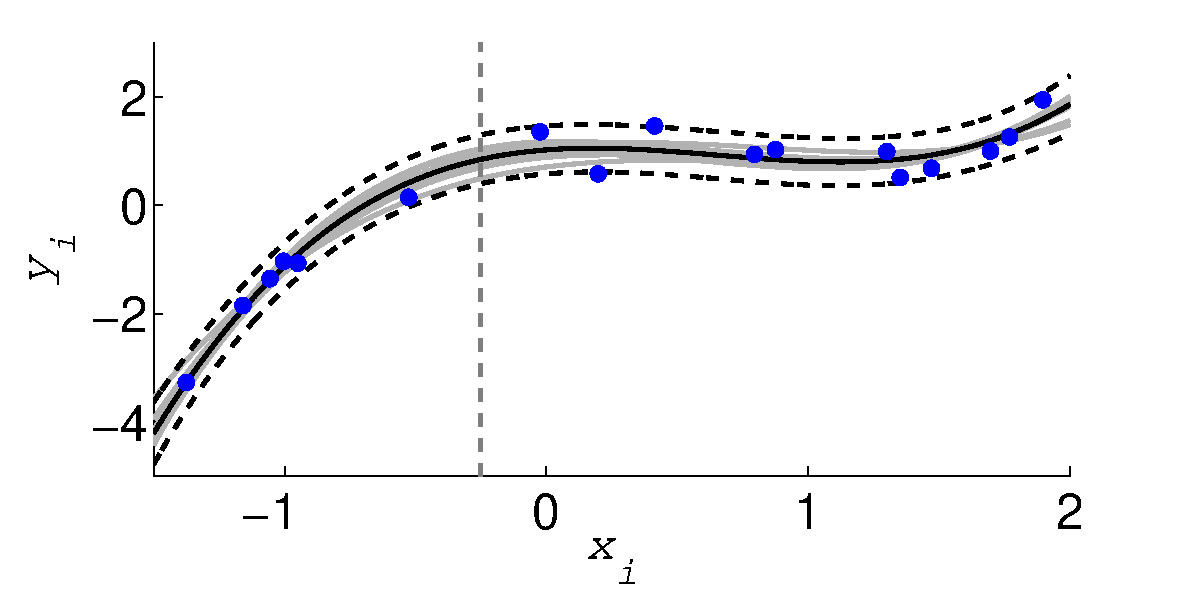
\includegraphics[width=0.6\textwidth]{polynomial_deg3_predictive_dist_and_post_samples}}

Remember that a finite linear model $f(x_n)=\bphi(x_n)^\top\bfw$ with prior on the weights 
$p(\bfw)=\N(\bfw;\; \mathbf{0}, \sigma_{\bm w}^2 \bfI)$ has a posterior distribution
\[
\Green{p(\bfw|\bfx,\bfy,\mathcal{M})}\;=\;\N(\bfw;\;\bmu,\,\bSigma)
\mathrm{\; \; \; with \; \; \;}
\begin{array}{l}
\bSigma\;=\;\left(\sigma_\mathrm{noise}^{-2}\bPhi^\top\bPhi+
  \sigma_{\bm w}^{-2}\right)^{-1}\\
\bmu\;=\;\Big(\bPhi^\top\bPhi+
  \frac{\sigma_\mathrm{noise}^2}{\sigma_{\bm w}^2}\,I\Big)^{-1}\bPhi^\top\bfy
\end{array}
\]
and predictive distribution
\[
p(y_*|x_*,\bfx, \bfy,\mathcal{M})\;=\;
\N(y_*;\; \bphi(x_*)^\top\bmu,\,\bphi(x_*)^\top\bSigma\bphi(x_*)+\sigma_\mathrm{noise}^2\,\bfI)
\]
\end{frame}



\begin{frame}
\frametitle{Marginal likelihood (Evidence) of our polynomials}

Marginal likelihood, or ''evidence'' of a finite linear model:
\[
\begin{split}
\Cyan{p(\bfy|\bfx,\mathcal{M})}\;&=\;
\int \Blue{p(\bfw|\mathcal{M})}
\Red{p(\bfy|\bfx,\bfw,\mathcal{M})}  d{\bf w}\\
&=\;\N(\bfy;\;\mathbf{0},\sigma_{\bm w}^2\,\bPhi\,\bPhi^\top+\sigma_\mathrm{noise}^2\,\bfI).
\end{split}
\]
Luckily for Gaussian noise there is a closed-form analytical solution!
%
\parbox{0.5\textwidth}{
\centerline{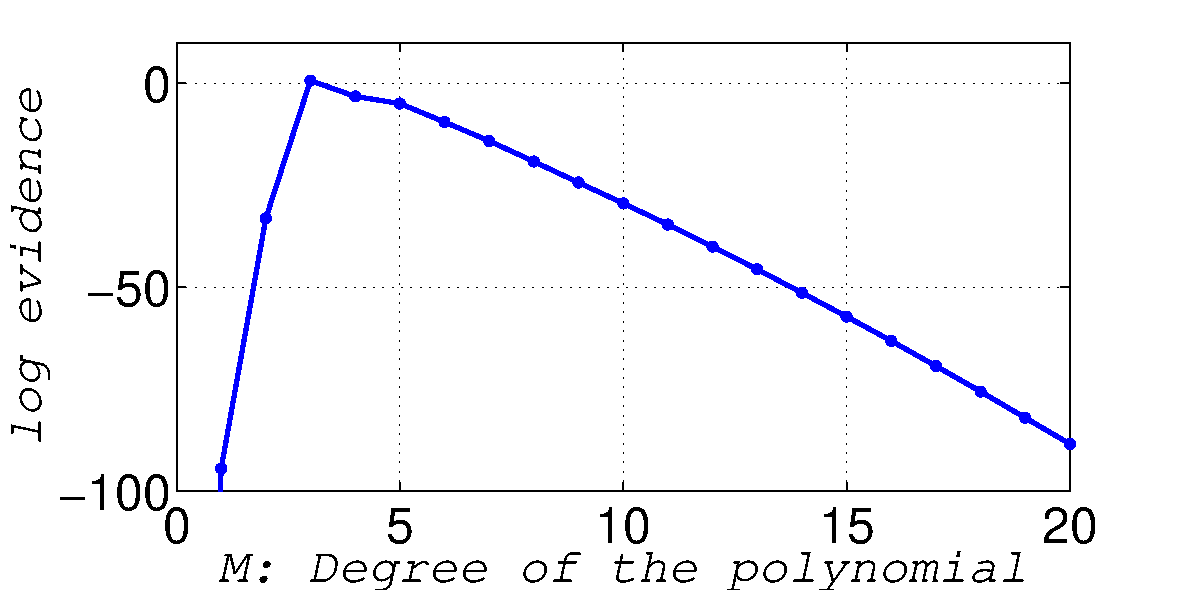
\includegraphics[width=0.51\textwidth]{polynomial_evidence}}
}
\hfill
\parbox{0.49\textwidth}{
\begin{itemize}
\item The evidence prefers $M=3$,\\ not simpler, not more complex.
\item Too simple models consistently miss most data.
\item Too complex models frequently miss some data.
\end{itemize}
}
\end{frame}

\end{document}
